\documentclass[9pt,a4paper,titlepage,oneside,mathserif,serif]{beamer}
\usepackage[latin1]{inputenc}
\usepackage{amsmath}
\usepackage{amsfonts}
\usepackage{amssymb}
\usepackage{graphicx}
\author{Leonhard Applis}
\title{Edge Detection}
\subtitle{}
\institute{TH N�rnberg} % (optional)
\date{05.11.2018}
\subject{AvBildMed}

\usetheme{PaloAlto}
\usecolortheme{beaver}
\AtBeginSection[]
{
	\begin{frame}
	\frametitle{Table of Contents}
	\tableofcontents[currentsection,currentsubsection]
\end{frame}
}

\begin{document}
\frame{\titlepage}
\section{What makes an Edge?}
\begin{frame}
	\frametitle{What makes an edge?}
	\begin{columns}
		\begin{column}{0.5\textwidth}
			\begin{figure}
				\centering
				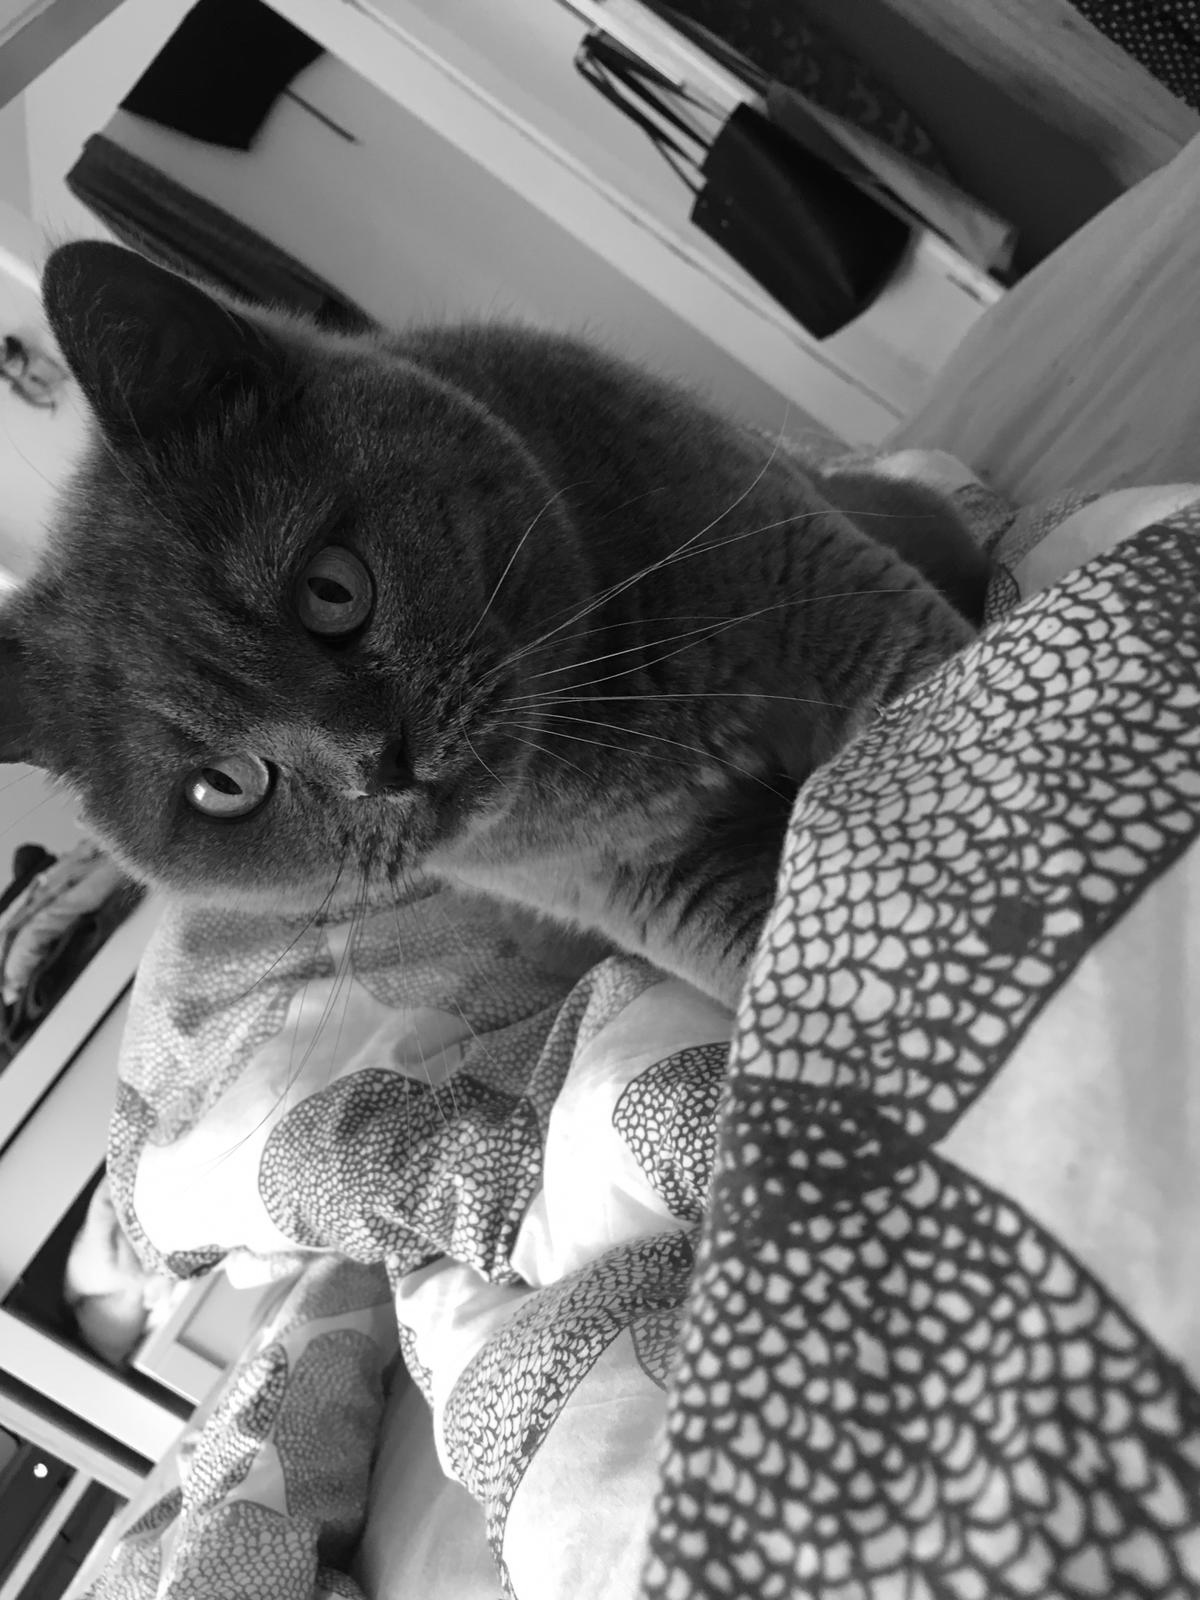
\includegraphics[width=0.8\linewidth]{images/Kadse}
				\caption[Felix]{Felix}
				\label{fig:kadse}
			\end{figure}
		\end{column}
		\begin{column}{0.5\textwidth}  %%<--- here
			\begin{center}
			\begin{figure}
				\centering
				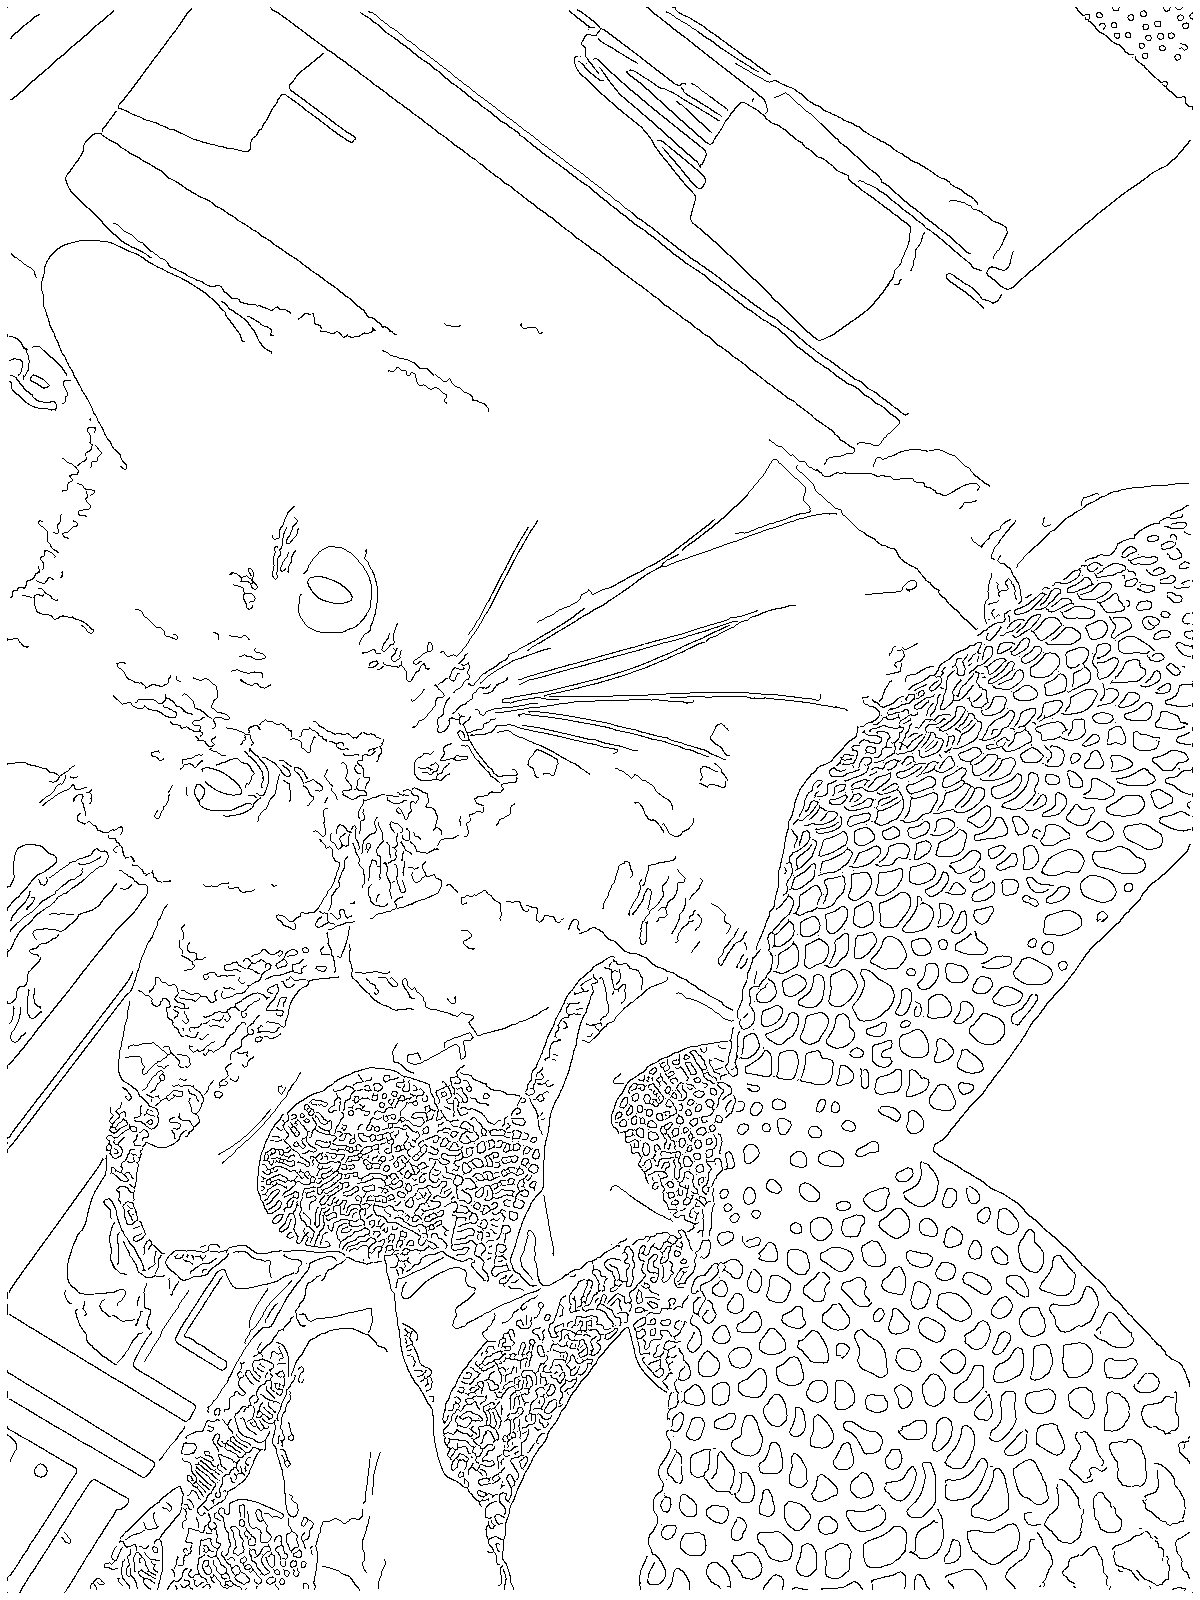
\includegraphics[width=0.8\linewidth]{images/KadseCanny}
				\caption[Felix's Edges]{Felix's Edges}
				\label{fig:kadseCanny}
			\end{figure}
			\end{center}
		\end{column}
	\end{columns}
\end{frame}
\subsection{Problems}
\begin{frame}
\frametitle{Problem I: Contrast}
\begin{columns}
	\begin{column}{0.5\textwidth}
		\begin{figure}
			\centering
			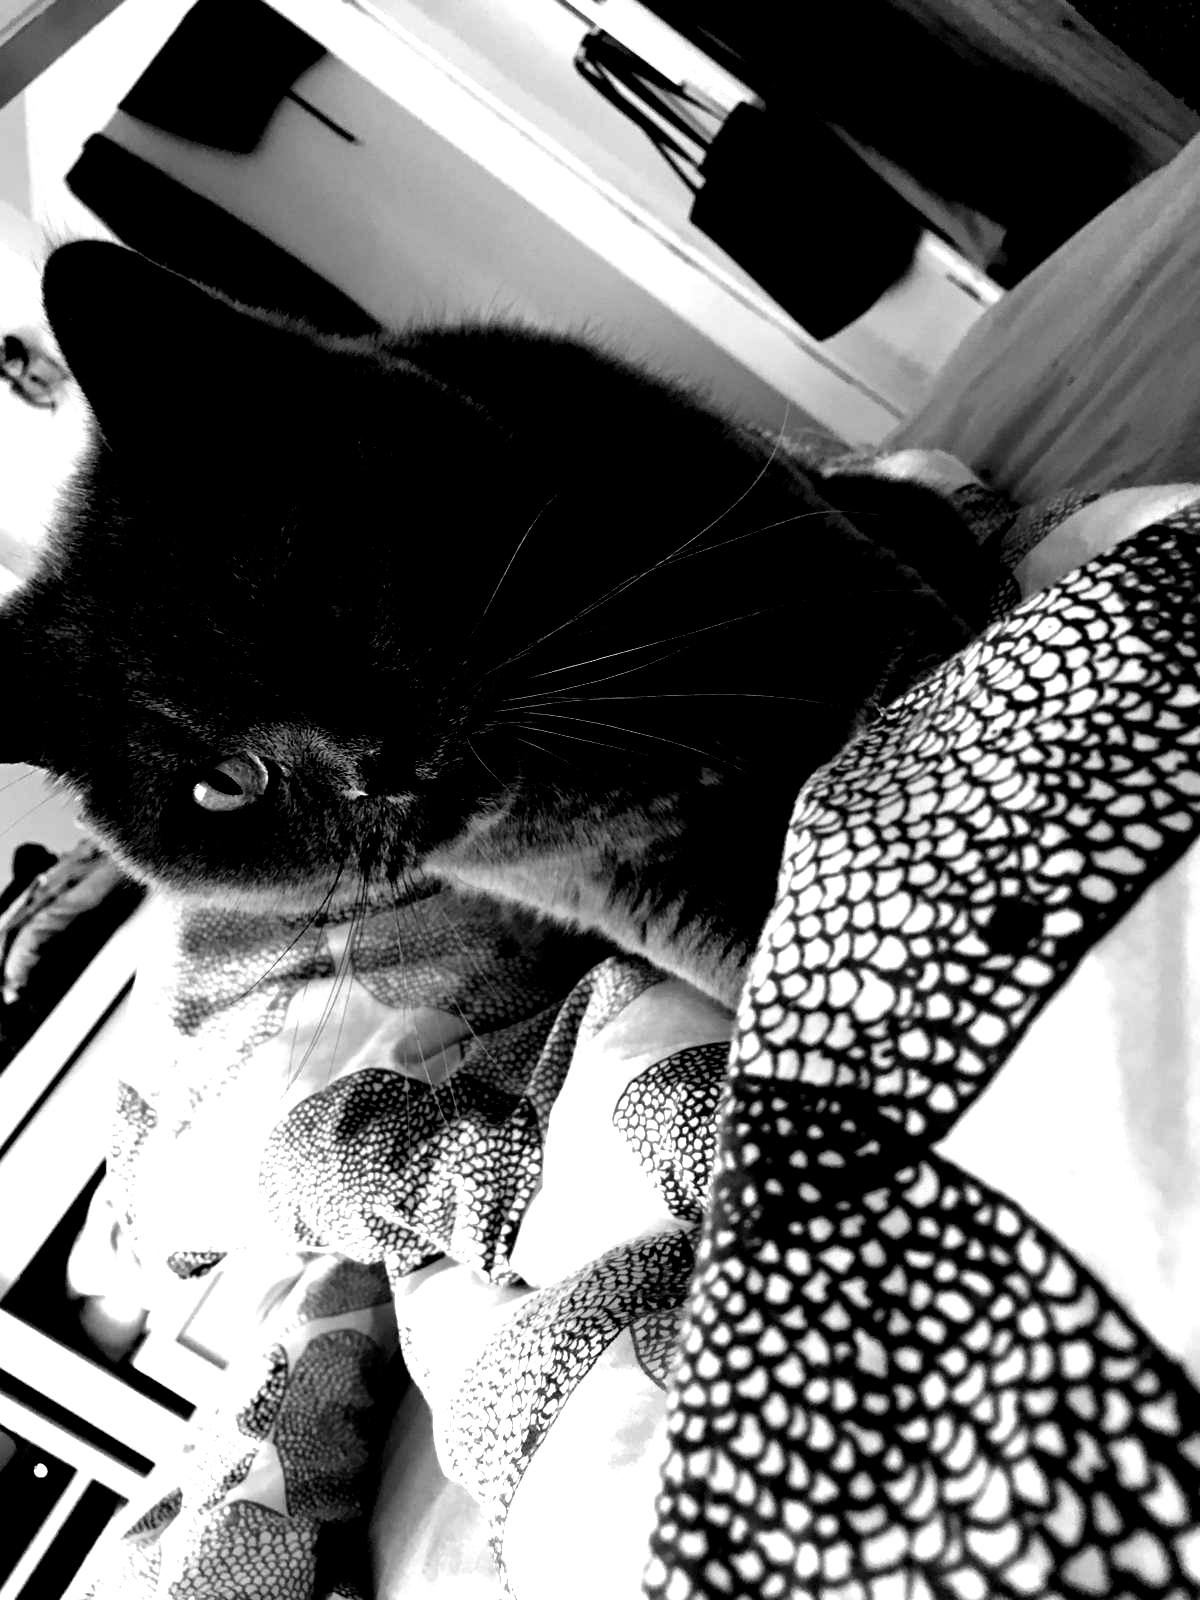
\includegraphics[width=0.8\linewidth]{images/KadseHighContrast}
			\caption[High Contrast Felix]{High Contrast Felix}
			\label{fig:HighContrast}
		\end{figure}
	\end{column}
	\begin{column}{0.5\textwidth}  %%<--- here
		\begin{center}
			\begin{figure}
				\centering
				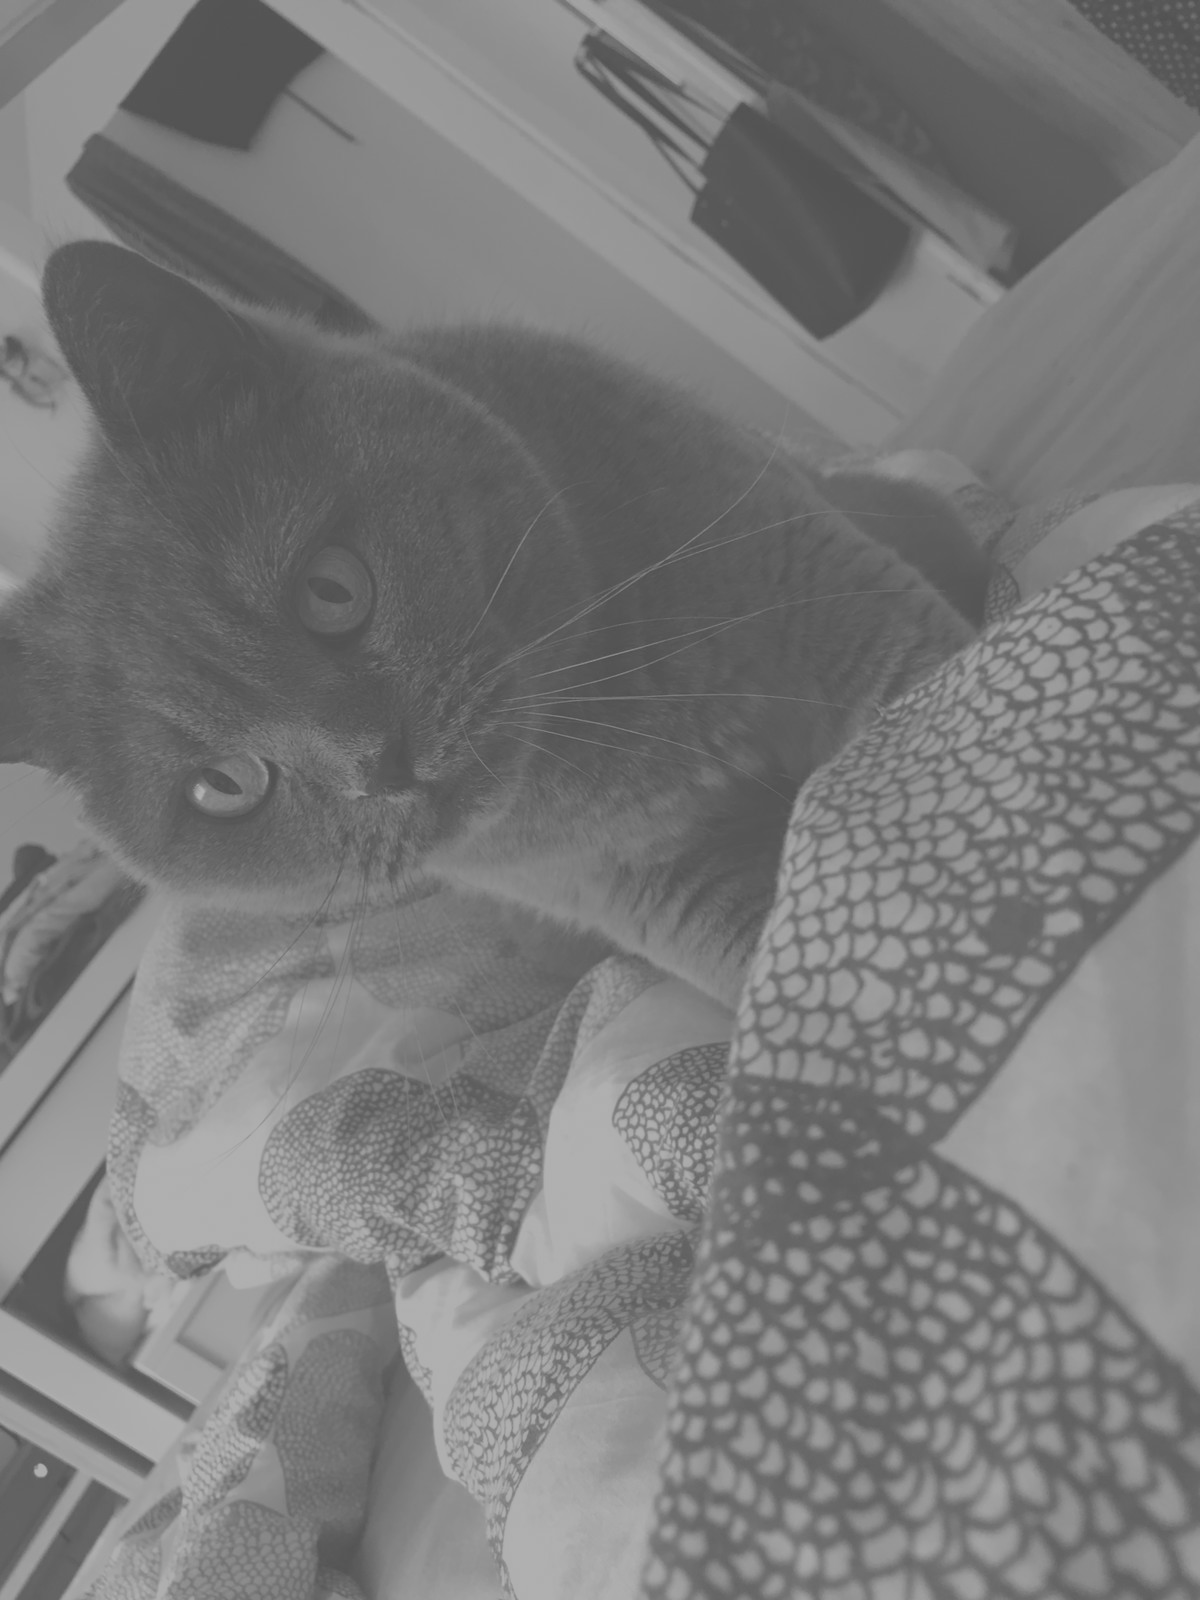
\includegraphics[width=0.8\linewidth]{images/KadseLowContrast}
				\caption[Low Contrast Felix]{Low Contrast Felix}
				\label{fig:LowContrast}
			\end{figure}
		\end{center}
	\end{column}
\end{columns}
\end{frame}

\begin{frame}
\frametitle{Problem II: Smoothness}
	\begin{center}
		\begin{figure}
			\centering
			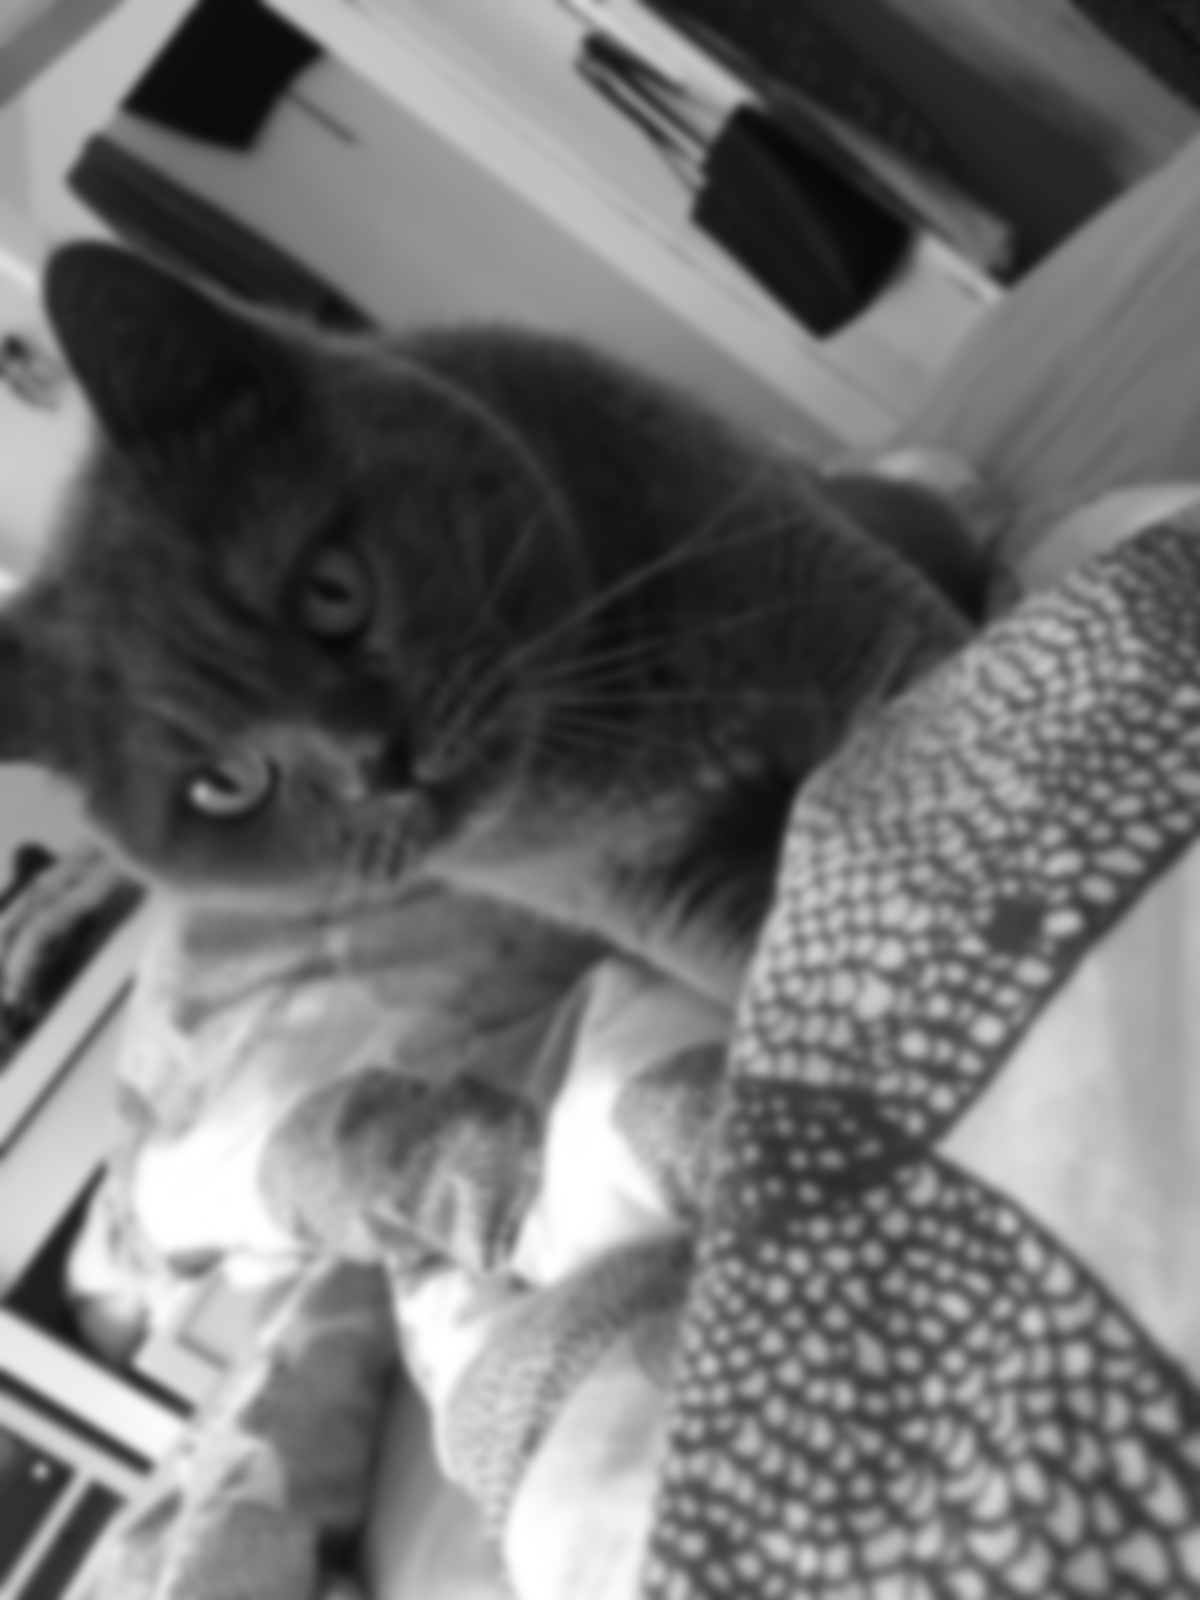
\includegraphics[width=0.4\linewidth]{images/KadseSmooth}
			\caption[Smooth Felix]{Smooth Felix}
			\label{fig:Smooth}
		\end{figure}
	\end{center}
\end{frame}

\begin{frame}
\frametitle{Problem III: Noise}
\begin{center}
	\begin{figure}
		\centering
		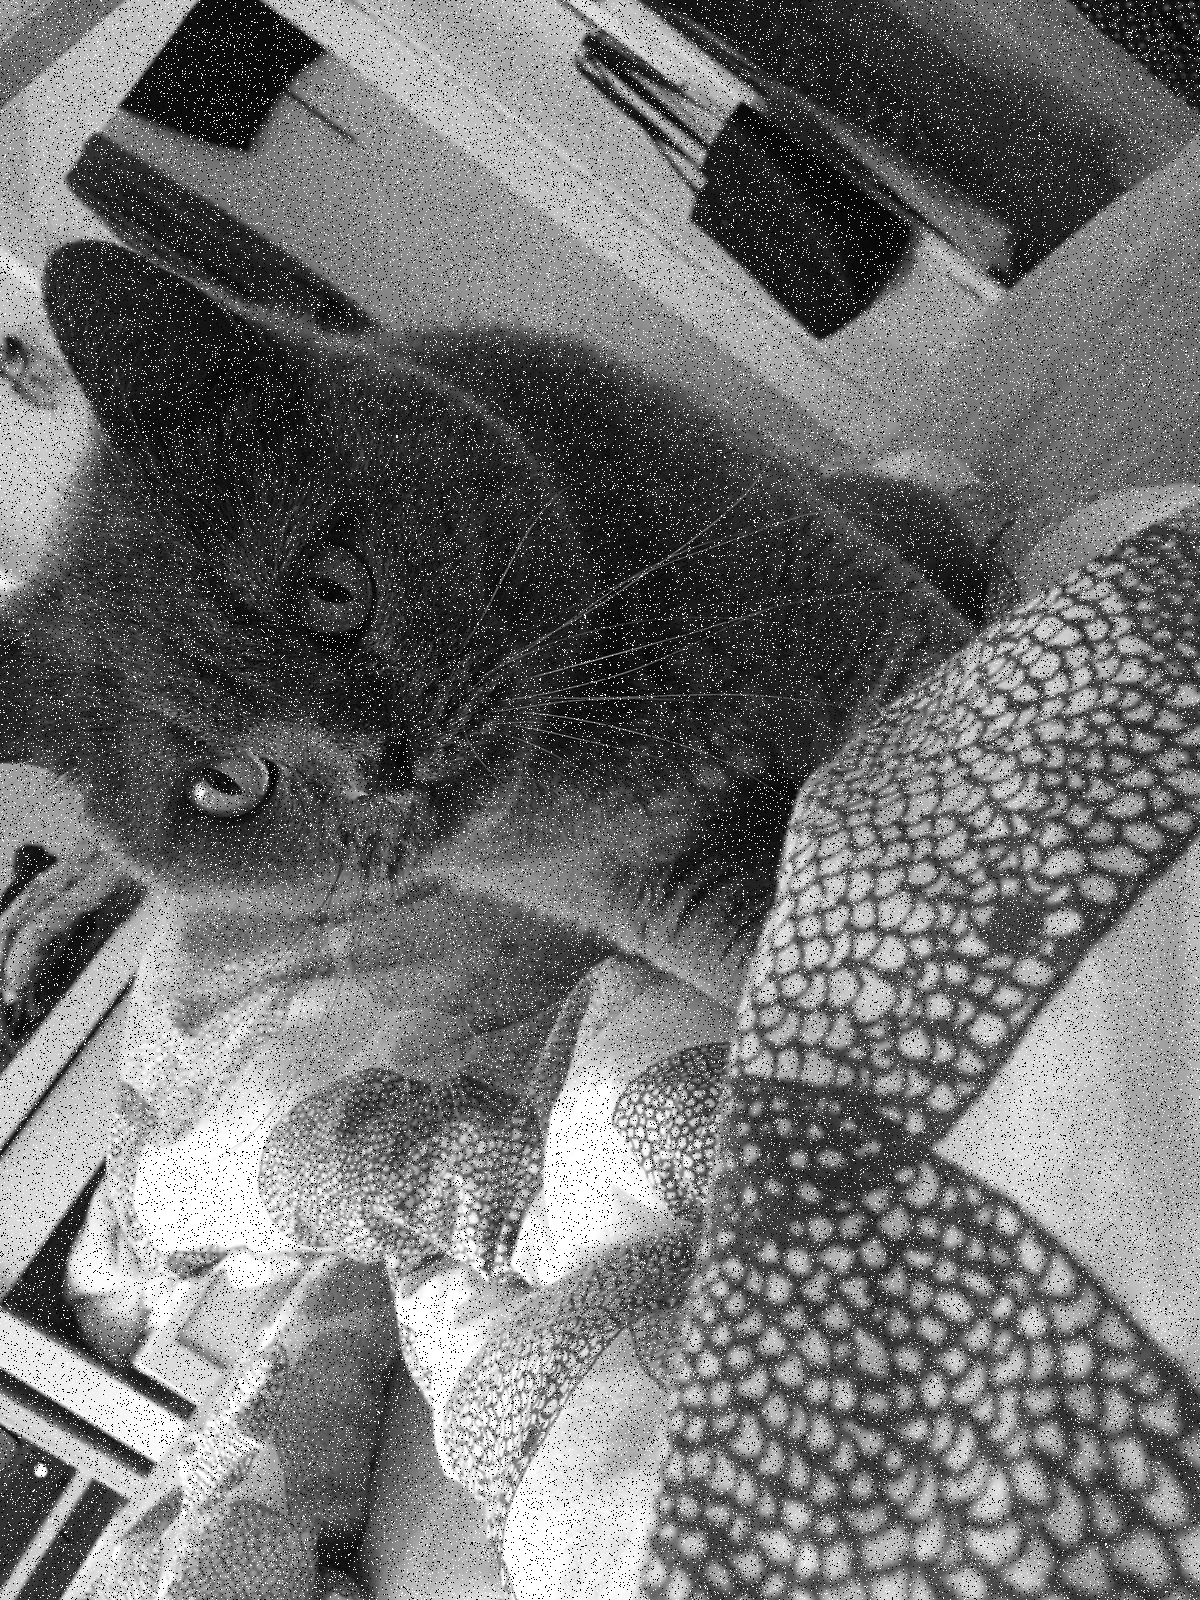
\includegraphics[width=0.4\linewidth]{images/KadseSalty}
		\caption[Salted Felix]{Salted Felix}
		\label{fig:Salted}
	\end{figure}
\end{center}
\end{frame}
\subsection{Definition}
\begin{frame}
	\frametitle{Definition}
	In Image Processing, an edge can be defined as a set of contiguous pixel positions where an abrupt change of intensity, gray- or color-values occur. Edges represent boundaries between objects and background. Sometimes, the edge-pixel-sequence may be broken due to insufficient intensity difference.(Malay K. Pakhira )
\end{frame}	
\section{Basics of gradient-based edgedetection}
\begin{frame}
\frametitle{Requirements}
\begin{enumerate}
	\item color values known (for examples only grayscale)
	\item picture scale known 
	\item loaded as pixelmatrix 
\end{enumerate}
\end{frame}	
\subsection{1D approach}
\begin{frame}
\frametitle{One dimensional approach}
\begin{center}
	\begin{figure}
		\centering
		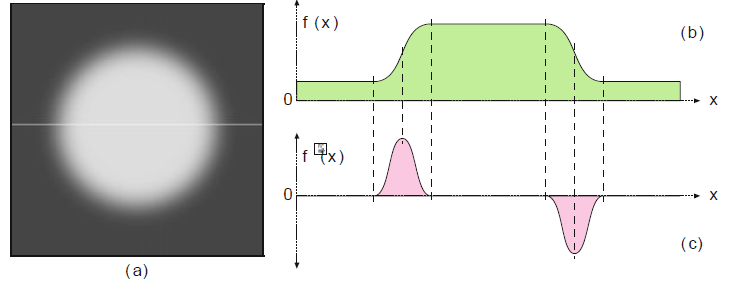
\includegraphics[width=0.7\linewidth]{images/1DGradient}
		\caption[1D Gradient]{One dimensional image function and derivation}
		\label{fig:1dgradient}
	\end{figure}
	\b{Only applyable with known, steady functions}
\end{center}
\end{frame}
\begin{frame}
\frametitle{Approximating discrete derivation}
Problem: the image function is discrete, therefore we need to approximate the derivation


\begin{center}
	\begin{figure}
		\centering
		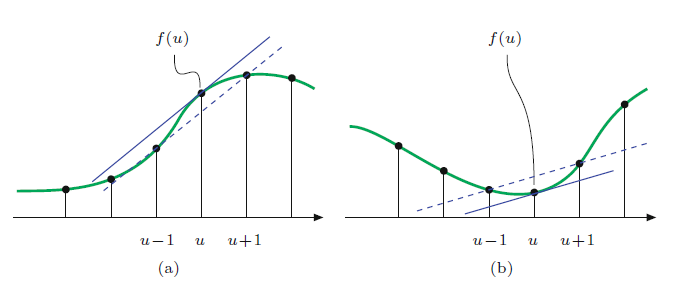
\includegraphics[width=0.7\linewidth]{images/1DGradientApproximation}
		\caption[1D Gradient Approximation]{Approximation of the derivation for discrete imagefunctions}
		\label{fig:1dgradientapprox}
	\end{figure}
	$\dfrac{df}{dx}(u) \approx \dfrac{f(u+1) - f(u-1)}{(u+1)-(u-1)} = \dfrac{f(u+1) - f(u-1)}{2}$
\end{center}
\end{frame}
\subsection{2D Approach}
\begin{frame}
	\frametitle{Two dimensional approach}
	If working with full images,we got two dimensions and therefore two partial derivations:
	\begin{center}	
		$I_x = \dfrac{\partial I}{\partial x}(u,v) , I_y = \dfrac{\partial I}{\partial y}(u,v)$
	\end{center}
	the \textbf{gradient} at the point \textit{(u,v)} is \newline
	\begin{center}
			$\nabla I(u,v) =  \begin{pmatrix}
		I_x(u,v) \\ I_y(u,v)
		\end{pmatrix}$
		
	\end{center}	
	\newline
	And the \textbf{magnitude} is \newline
	\begin{center}
		$|\nabla I|=\sqrt{I_x^2 + I_y^2}$
	\end{center}
	~\newline
\end{frame}

\begin{frame}
	\frametitle{Example}
	\begin{figure}
		\centering
		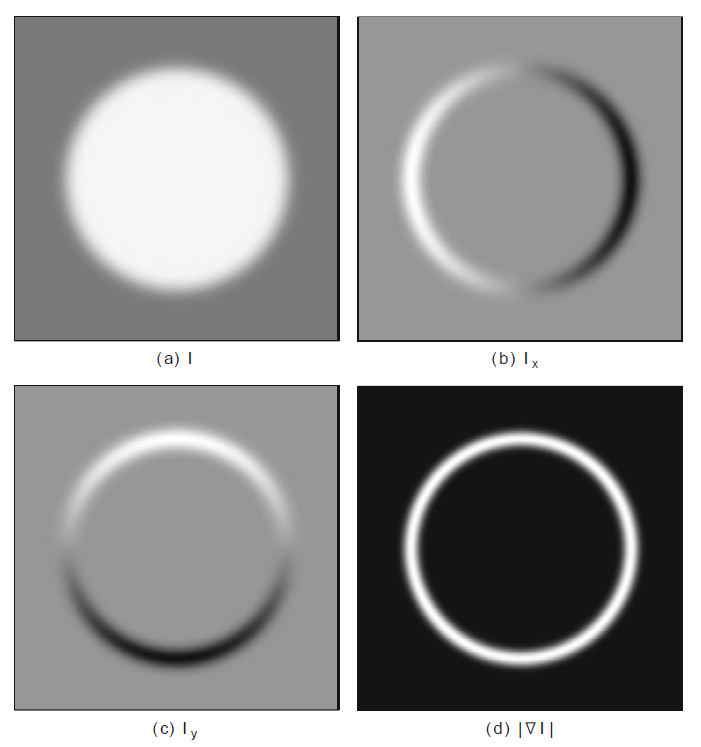
\includegraphics[width=0.8\linewidth]{images/2DEdgeGradient}
		\caption{}
		\label{fig:2dedgegradient}
	\end{figure}
\end{frame}
\subsection{Filters}
\begin{frame}
	\frametitle{Implementation with filters}
	Expressing the gradient as a \textit{linear filter} is simple:
	\begin{center}
			$I_x = \begin{bmatrix}
		-0.5 & 0 & 0.5
		\end{bmatrix}
		I_y = \begin{bmatrix}
		-0.5 \\ 0 \\ 0.5
		\end{bmatrix}$
	\end{center}
\end{frame}
\section{Advanced gradient-based edgedetection}

\section{Compass Operators}

\section{Edge Sharpening}

\end{document}